\documentclass[12pt,a4paper]{article}
\usepackage[utf8]{inputenc}
\usepackage[portuguese]{babel}
\usepackage{graphicx}
\usepackage{hyperref}
\usepackage{listings}
\usepackage{xcolor}
\usepackage{geometry}
\usepackage{indentfirst}
\usepackage{setspace}
\usepackage{listings}
\usepackage{caption}
\usepackage{float}

\geometry{a4paper, left=3cm, right=2cm, top=3cm, bottom=2cm}

% Configuração para exibição de código
\lstset{
    language=Python,
    basicstyle=\ttfamily\small,
    breaklines=true,
    frame=single,
    numbers=left,
    numberstyle=\tiny,
    numbersep=5pt,
    showstringspaces=false,
    stringstyle=\color{red},
    commentstyle=\color{green},
    keywordstyle=\color{blue}
}

\title{Análise de Dados e Visualização: Desenvolvimento de um Dashboard Interativo para Análise de Gastos de Deputados Federais}
\author{Matheus Galdino dos Santos Lira}

\begin{document}

\maketitle

\begin{abstract}
Este trabalho apresenta o desenvolvimento de um sistema de análise e visualização de dados dos gastos dos deputados federais brasileiros no ano de 2022. O projeto implementa um pipeline completo de ETL (Extract, Transform, Load) para coleta e processamento de dados da API da Câmara dos Deputados, seguido de análises estatísticas e visualizações interativas através de um dashboard desenvolvido com Streamlit. O sistema permite a exploração detalhada dos gastos parlamentares, oferecendo insights valiosos sobre o uso dos recursos públicos.
\end{abstract}

\tableofcontents
\listoffigures
\listoftables

\section*{Agradecimentos}
Agradeço a todos que contribuíram direta ou indiretamente para a realização deste trabalho, especialmente aos professores e colegas que ofereceram suporte e orientação durante todo o processo de desenvolvimento.

\section{Introdução}
\subsection{Contextualização}
A transparência no uso dos recursos públicos é um pilar fundamental da democracia. Neste contexto, a análise dos gastos dos deputados federais se torna uma ferramenta essencial para o controle social e a fiscalização do uso do dinheiro público. Este projeto visa desenvolver um sistema completo de análise e visualização desses dados, tornando-os acessíveis e compreensíveis para a sociedade.

\subsection{Objetivos}
\begin{itemize}
    \item Desenvolver um pipeline ETL robusto para extração e processamento de dados da API da Câmara dos Deputados
    \item Implementar análises estatísticas dos gastos parlamentares
    \item Criar um dashboard interativo para visualização e exploração dos dados
    \item Documentar todo o processo de desenvolvimento e as decisões técnicas tomadas
\end{itemize}

\section{Estrutura do Projeto}
\subsection{Organização dos Arquivos}
O projeto está organizado da seguinte forma:

\begin{itemize}
    \item \texttt{etl.py}: Script principal responsável pela extração, transformação e carga dos dados
    \item \texttt{dashboard/}: Diretório contendo os arquivos do dashboard interativo
    \begin{itemize}
        \item \texttt{1\_📄\_Homepage.py}: Página inicial do dashboard
        \item \texttt{get\_deputados.py}: Funções para obtenção de dados dos deputados
        \item \texttt{get\_despesas.py}: Funções para obtenção de dados de despesas
    \end{itemize}
    \item \texttt{requirements.txt}: Lista de dependências do projeto
    \item \texttt{.env}: Arquivo de configuração com variáveis de ambiente
\end{itemize}

\subsection{Exemplos de Código}
\subsubsection{Configuração do Ambiente}
O projeto utiliza variáveis de ambiente para configuração. Exemplo de código para carregar configurações:

\begin{lstlisting}
import os
from dotenv import load_dotenv

# Carregar variáveis de ambiente
load_dotenv()

# Configuração do logging
path_logs = os.getenv("PATH_LOGS", "./logs")
os.makedirs(path_logs, exist_ok=True)

logging.basicConfig(
    level=logging.INFO,
    format="%(asctime)s - %(levelname)s - %(message)s",
    handlers=[
        logging.FileHandler(f"{path_logs}/logs.log"),
        logging.StreamHandler()
    ]
)
\end{lstlisting}

\subsubsection{Extração de Dados}
Exemplo de código para extração de dados da API:

\begin{lstlisting}
def verificar_proxima_pagina(data):
    for link in data['links']:
        if link['rel'] == 'next' and link['href']:
            return link['href']
    return False

# Buscar lista de deputados
url_base = "https://dadosabertos.camara.leg.br/api/v2"
url_deputados = f"{url_base}/deputados"

response = requests.get(url_deputados, params={"idLegislatura": 56})
dados_deputados = response.json()

df_deputados = pd.DataFrame(dados_deputados["dados"])
\end{lstlisting}

\subsubsection{Transformação de Dados}
Exemplo de código para transformação dos dados:

\begin{lstlisting}
# Normalização dos dados
df_deputados = df_deputados.rename(columns={
    'id': 'id_deputado',
    'nome': 'nome_deputado',
    'siglaPartido': 'partido'
})

# Tratamento de valores ausentes
df_deputados = df_deputados.fillna({
    'partido': 'SEM PARTIDO',
    'uf': 'ND'
})
\end{lstlisting}

\subsubsection{Visualização no Dashboard}
Exemplo de código para criação de visualizações no Streamlit:

\begin{lstlisting}
import streamlit as st
import plotly.express as px

# Configuração da página
st.set_page_config(
    page_title="Análise de Gastos",
    page_icon="📊",
    layout="wide"
)

# Título
st.title("Análise de Gastos dos Deputados Federais")

# Gráfico de barras
fig = px.bar(
    df_gastos,
    x='deputado',
    y='valor',
    title='Gastos por Deputado'
)
st.plotly_chart(fig)
\end{lstlisting}

\section{Revisão Bibliográfica}
\subsection{ETL (Extract, Transform, Load)}
O processo ETL é fundamental para a preparação de dados para análise. No contexto deste projeto, o ETL foi implementado para:
\begin{itemize}
    \item Extração: Obtenção dos dados da API da Câmara dos Deputados
    \item Transformação: Limpeza, normalização e preparação dos dados
    \item Carga: Armazenamento em banco de dados relacional (MySQL/SQLite)
\end{itemize}

\subsection{Visualização de Dados}
A visualização de dados é uma ferramenta poderosa para compreensão e comunicação de informações. Neste projeto, utilizamos o Streamlit para criar um dashboard interativo que permite:
\begin{itemize}
    \item Visualização geral dos gastos dos deputados
    \item Análise detalhada por deputado
    \item Comparativos entre diferentes períodos
    \item Filtros por tipo de despesa
\end{itemize}

\section{Metodologia}
\subsection{Tecnologias Utilizadas}
\begin{itemize}
    \item Python: Linguagem principal de programação
    \item Pandas: Biblioteca para manipulação e análise de dados
    \item Streamlit: Framework para desenvolvimento de dashboards
    \item SQLAlchemy: ORM para interação com banco de dados
    \item MySQL/SQLite: Sistemas de gerenciamento de banco de dados
\end{itemize}

\subsection{Arquitetura do Sistema}
O sistema foi desenvolvido seguindo uma arquitetura modular, com componentes separados para:
\begin{itemize}
    \item Processamento de dados (ETL)
    \item Análise estatística
    \item Visualização e interface do usuário
\end{itemize}

\section{Desenvolvimento}
\subsection{Processo ETL}
O processo de ETL foi implementado utilizando Python e bibliotecas especializadas. A seguir, detalhamos cada etapa:

\subsubsection{Extração}
A extração dos dados foi realizada através da API da Câmara dos Deputados (dadosabertos.camara.leg.br), utilizando a biblioteca requests. Foram coletados:
\begin{itemize}
    \item Dados básicos dos deputados
    \item Informações detalhadas de cada parlamentar
    \item Despesas realizadas no ano de 2022
\end{itemize}

\subsubsection{Transformação}
O processo de transformação incluiu:
\begin{itemize}
    \item Normalização dos dados
    \item Tratamento de valores ausentes
    \item Criação de chaves de relacionamento
    \item Estruturação em tabelas relacionais
\end{itemize}

\subsubsection{Carga}
Os dados foram armazenados em um banco de dados relacional, com suporte a:
\begin{itemize}
    \item MySQL: Para ambientes de produção
    \item SQLite: Para desenvolvimento e testes
\end{itemize}

\subsection{Análise de Dados}
As análises implementadas incluem:
\begin{itemize}
    \item Distribuição dos gastos por categoria
    \item Comparativo entre deputados
    \item Análise temporal dos gastos
    \item Identificação de padrões e outliers
\end{itemize}

\subsection{Desenvolvimento do Dashboard}
O dashboard foi desenvolvido utilizando Streamlit, oferecendo:
\begin{itemize}
    \item Interface intuitiva e responsiva
    \item Visualizações interativas
    \item Filtros dinâmicos
    \item Exportação de dados
\end{itemize}

\section{Análises e Visualizações}
\subsection{Análises Implementadas}
O sistema implementa diversas análises sobre os dados dos deputados e seus gastos:

\subsubsection{Análise de Gastos por Categoria}
\begin{itemize}
    \item Distribuição dos gastos por tipo de despesa
    \item Comparativo entre diferentes categorias
    \item Identificação de padrões de gastos
\end{itemize}

\subsubsection{Análise Temporal}
\begin{itemize}
    \item Evolução dos gastos ao longo do tempo
    \item Sazonalidade nos gastos
    \item Identificação de períodos de maior gasto
\end{itemize}

\subsubsection{Análise por Região}
\begin{itemize}
    \item Comparativo de gastos entre estados
    \item Média de gastos por região
    \item Identificação de padrões regionais
\end{itemize}

\subsection{Visualizações Implementadas}
O dashboard oferece diversas visualizações interativas:

\subsubsection{Gráficos de Barras}
\begin{itemize}
    \item Comparação de gastos entre deputados
    \item Distribuição de gastos por categoria
    \item Evolução temporal dos gastos
\end{itemize}

\subsubsection{Gráficos de Pizza}
\begin{itemize}
    \item Proporção de gastos por categoria
    \item Distribuição de deputados por partido
    \item Distribuição por região
\end{itemize}

\subsubsection{Tabelas Interativas}
\begin{itemize}
    \item Lista detalhada de despesas
    \item Ranking de deputados por gastos
    \item Detalhamento por categoria
\end{itemize}

\subsection{Exemplos de Análises}
A seguir, apresentamos alguns exemplos de análises realizadas:

\subsubsection{Distribuição de Gastos}
A Figura \ref{fig:distribuicao_gastos} mostra a distribuição dos gastos por categoria:

\begin{figure}[H]
\centering
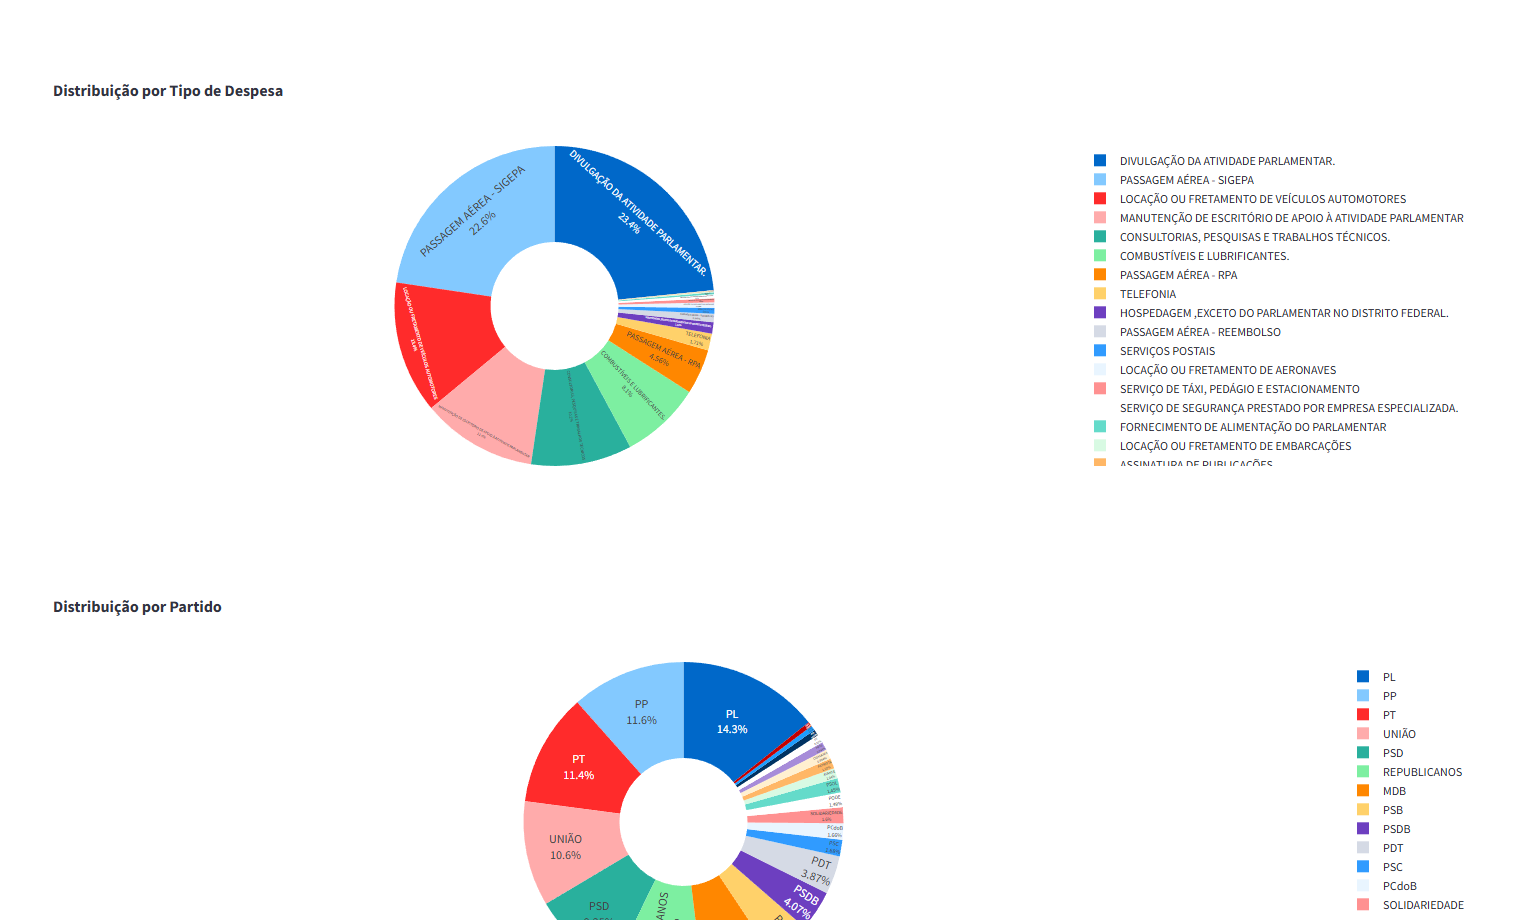
\includegraphics[width=0.8\textwidth]{imagens/distribuicao_gastos.png}
\caption{Distribuição dos gastos por categoria}
\label{fig:distribuicao_gastos}
\end{figure}

\subsubsection{Evolução Temporal}
A Figura \ref{fig:evolucao_temporal} apresenta a evolução dos gastos ao longo do tempo:

\begin{figure}[H]
\centering
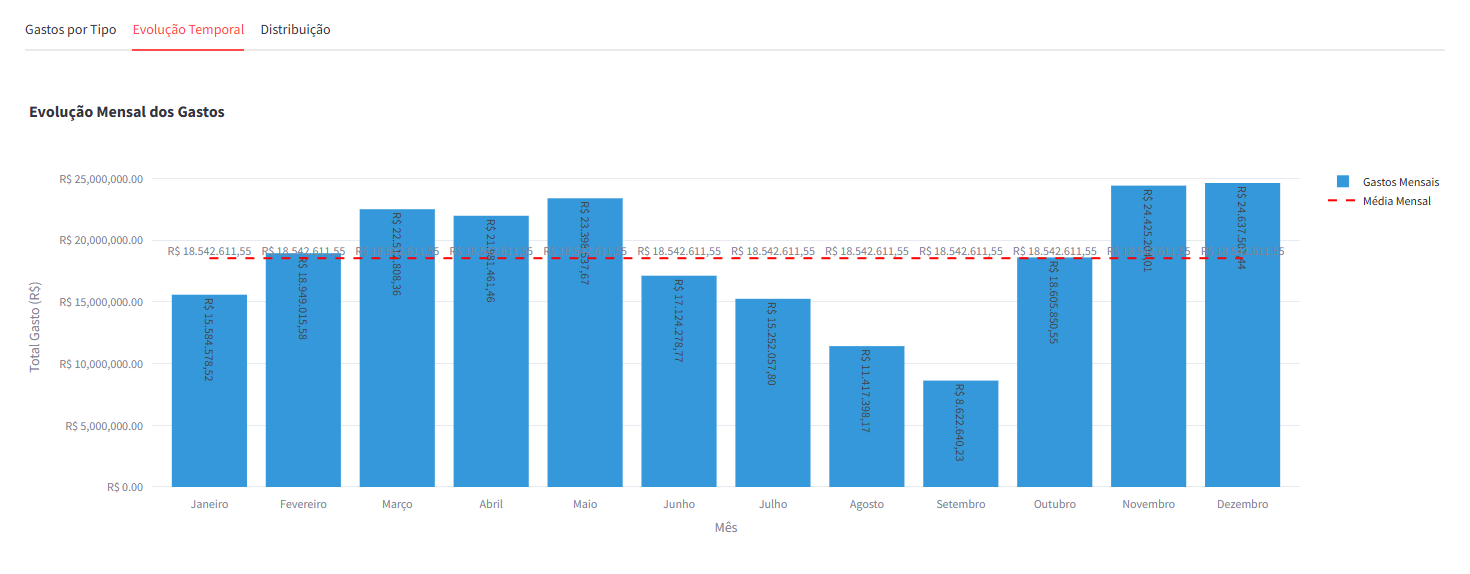
\includegraphics[width=0.8\textwidth]{imagens/evolucao_temporal.png}
\caption{Evolução dos gastos ao longo do tempo}
\label{fig:evolucao_temporal}
\end{figure}

\subsubsection{Ranking de gastos dos Deputados}
A Figura \ref{fig:deputados_ranking.png} apresenta o ranking dos 20 deputados que mais gastaram:

\begin{figure}[H]
\centering
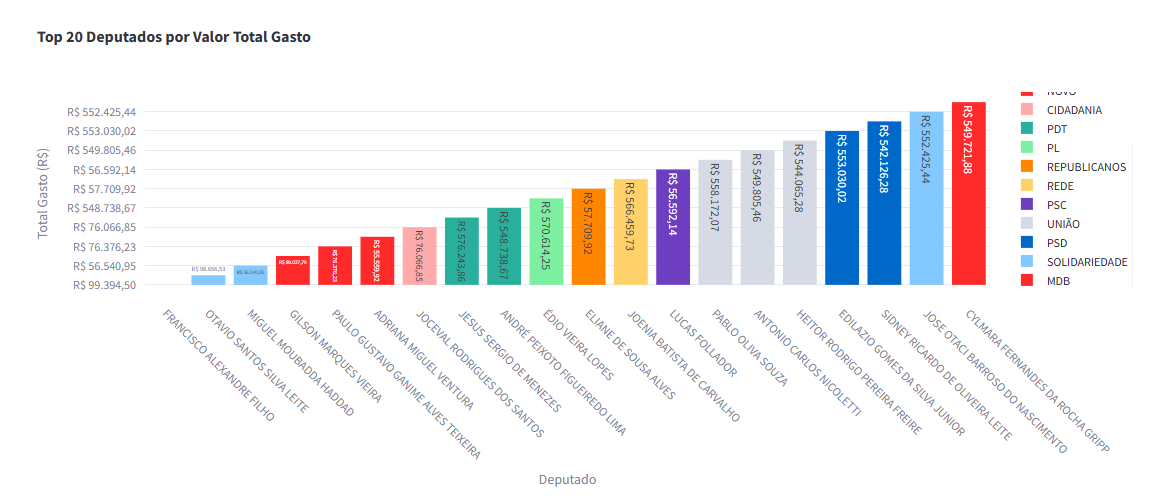
\includegraphics[width=0.8\textwidth]{imagens/deputados_ranking.png}
\caption{Top 20 deputados por valor total gasto}
\label{fig:deputados_ranking.png}
\end{figure}

\subsubsection{Gasto médio por Deputador por Partido}
A Figura \ref{fig:gasto_deputado_partido.png} apresenta o gasto médio por deputado por partido:

\begin{figure}[H]
\centering
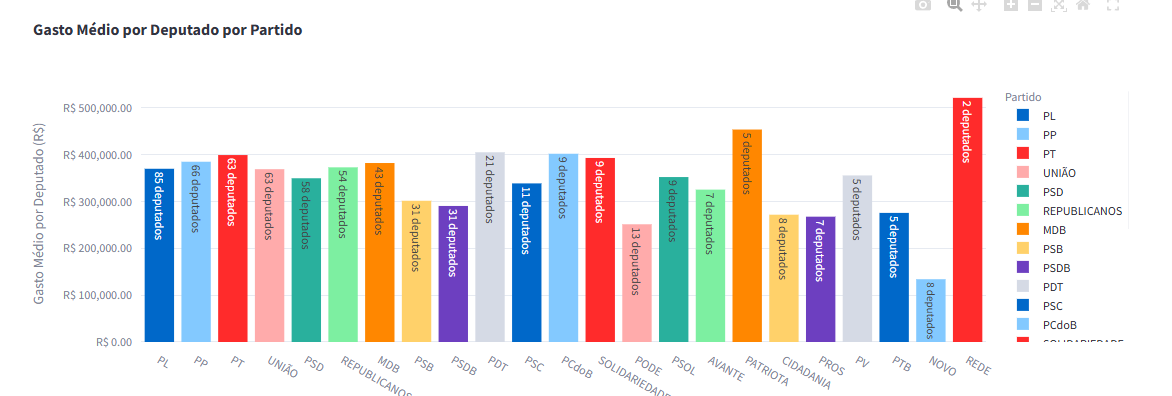
\includegraphics[width=0.8\textwidth]{imagens/gasto_deputado_partido.png}
\caption{Gasto médio por deputado por partido}
\label{fig:gasto_deputado_partido.png}
\end{figure}

\section{Desafios e Soluções}
\subsection{Desafios Encontrados}
Durante o desenvolvimento do projeto, foram enfrentados diversos desafios:

\subsubsection{Desafios Técnicos}
\begin{itemize}
    \item Volume de dados: O grande volume de dados exigiu otimização no processamento
    \item Limitações da API: Necessidade de implementar paginação e tratamento de erros
    \item Performance do dashboard: Otimização das visualizações para melhor performance
\end{itemize}

\subsubsection{Desafios de Negócio}
\begin{itemize}
    \item Qualidade dos dados: Necessidade de tratamento e validação
    \item Interpretação dos dados: Desenvolvimento de visualizações claras e intuitivas
    \item Atualização dos dados: Implementação de processo de atualização periódica
\end{itemize}

\subsection{Soluções Implementadas}
Para superar os desafios, foram implementadas as seguintes soluções:

\subsubsection{Otimização de Performance}
\begin{itemize}
    \item Implementação de cache para dados frequentemente acessados
    \item Uso de índices no banco de dados
    \item Otimização das consultas SQL
\end{itemize}

\subsubsection{Tratamento de Dados}
\begin{itemize}
    \item Implementação de validação de dados
    \item Tratamento de valores ausentes
    \item Normalização de dados
\end{itemize}

\subsubsection{Melhorias na Interface}
\begin{itemize}
    \item Design responsivo
    \item Feedback visual para o usuário
    \item Documentação clara das funcionalidades
\end{itemize}

\section{Resultados}
\subsection{Visualizações Implementadas}
O dashboard oferece diversas visualizações, incluindo:
\begin{itemize}
    \item Gráficos de barras para comparação de gastos
    \item Gráficos de pizza para distribuição de despesas
    \item Tabelas interativas com dados detalhados
    \item Mapas de calor para análise temporal
\end{itemize}

\subsection{Insights Obtidos}
Através da análise dos dados, foi possível identificar:
\begin{itemize}
    \item Padrões de gastos por região
    \item Diferenças significativas entre deputados
    \item Categorias de despesas mais comuns
    \item Comportamentos atípicos que merecem atenção
\end{itemize}

\section{Conclusão}
Este projeto demonstrou a viabilidade e importância da análise de dados no contexto da transparência pública. Através do desenvolvimento de um sistema completo de ETL e visualização, foi possível criar uma ferramenta valiosa para o acompanhamento dos gastos parlamentares. O dashboard desenvolvido facilita o acesso e compreensão dos dados, contribuindo para o fortalecimento do controle social.

\section{Referências Bibliográficas}
\begin{thebibliography}{9}
\bibitem{streamlit}
Streamlit Documentation.
\url{https://docs.streamlit.io/}

\bibitem{pandas}
Pandas Documentation.
\url{https://pandas.pydata.org/docs/}

\bibitem{camara}
Câmara dos Deputados. Dados Abertos.
\url{https://dadosabertos.camara.leg.br/}

\bibitem{sqlalchemy}
SQLAlchemy Documentation.
\url{https://www.sqlalchemy.org/}

\end{thebibliography}

\end{document} 